\newpage 
\section{Auswertung}

\noindent
Um die unterschiedlichen Relaxationszeiten und die Diffusionskonstanten zu bestimmen muss der Aufbau zuerst justiert werden. 
Dabei wir zuerst die Frequenz des \enquote{rotating frames}, welches ungefähr der Lamor-Frequenz entspricht, und die Phase eingestellt. Dies führt zu 
\begin{align*}
  \omega &= \SI{21.74}{\mega\hertz}\\
  \phi &= \SI{104.0}{\degree} \quad .
\end{align*}
Des Weiteren wurden die Pulslägen für den $\SI{90}{\degree}$- und den $\SI{180}{\degree}$-Puls bestimmt. Dafür ergeben sich
\begin{align*}
  \symup{\Delta} t_{90} &= \SI{2.64}{\micro\second}\\
  \symup{\Delta} t_{180} &= \SI{5.28}{\micro\second} \quad .
\end{align*}
Außerdem wurde zu allen Zeitpunkten dieselbe Temperatur 
\begin{equation*}
  T = \SI{20.8}{\degreeCelsius}
\end{equation*}
gemessen.


\subsection{Bestimmung der Spin-Gitter Relaxationszeit}

\noindent
Die zur Bestimmung der Spin-Gitter Relaxationszeit gemessenen Spannungsamplituden und ihre korrespondierenden Pulsabstände $\tau$ sind in Tabelle \ref{tab:T1} und in Abbildung \ref{img:T1} zu finden.\\
Auf die Messdaten wird eine Ausgleichsfunktion der Form 
\begin{equation*}
  U\left(\tau\right) = U_0 \left(1-2\exp{\left(-\frac{\tau}{T_1}\right)}\right) + U_1
\end{equation*}
gefittet. Für die Parameter ergibt sich dabei
\begin{align*}
  U_0 &= \SI{-1.60(1)}{\volt}\\
  T_1 &= \SI{2839.88(6789)}{\milli\second}\\
  U_1 &= \SI{-0.64(17)}{\volt} \quad .
\end{align*}
Der Fit ist dabei inklusive der Spannungsamplituden in Abbildung \ref{img:T1} grafisch dargestellt.

\begin{figure}[H]
  \centering
  \includegraphics[width=0.6\textwidth]{build/plots/T1.pdf}
  \caption{Die Messdaten der $T1$-Messung gegen die halblogarithmischen Pulsabstände aufgetragen. 
  Zusätzlich ist noch der mit damit korrespondierende Fit aufgetragen.}
\label{img:T1}
\end{figure}

\begin{table}[ht]
  \centering
  \small
  \caption{Die Messwerte der Spannungsamplituden $U$ und ihre korrespondierenden Pulsabstände $\tau$ für die $T_1$-Messung.}
  \label{tab:T1}
  \begin{tabular}{S [table-format=4.1] S [table-format=1.4] | S [table-format=4.1] S [table-format=1.4]}
   \toprule
   {$\tau \mathbin{\scalebox{1.5} / } \si{\milli\second}$} & $\text{Spannungsamplitude} \mathbin{\scalebox{1.5} / } \si{\volt}$ &{$\tau \mathbin{\scalebox{1.5} / } \si{\milli\second}$} & $\text{Spannungsamplitude} \mathbin{\scalebox{1.5} / } \si{\volt}$\\
   \midrule
   1   &  1.5375 &  150   &  1.36   \\
   1.5 &  1.525  &  300   &  1.2    \\
   2   &  1.525  &  500   &  1      \\
   3   &  1.525  &  750   &  0.72   \\
   5   &  1.55   & 1000   &  0.6    \\
   7.5 &  1.55   & 1400   &  0.375  \\
  10   &  1.5375 & 1800   &  0.11   \\
  15   &  1.5375 & 2300   & -0.26   \\
  20   &  1.525  & 3000   & -0.57   \\
  27.5 &  1.52   & 4500   & -1.085  \\
  35   &  1.5    & 6000   & -1.275  \\
  45   &  1.4875 & 7500   & -1.425  \\
  60   &  1.4625 & 9999   & -1.55   \\
  75   &  1.4375  & &\\
  \end{tabular}
\end{table} 


\subsection{Bestimmung der Spin-Spin Relaxationszeit}


\noindent
Für die Spin-Spin Relaxationszeit $T_2$ wird zunächst die Meiboom-Gill-Methode angewendet um $T_2$ zu berechnen. 
Anschließend wird das Signal der Carr-Purcell-Mehode gezeigt.

\subsubsection{Meiboom-Gill-Methode}

\noindent
Zur Bestimmung der Spin-Spin Relaxationszeit wurden mit der Funktion \textit{scipy.find\_peaks} die Maxima der $T_2$-Messreihe ausgelesen. 
Die ursprüngliche Messreihe umfasst $\approx 20000$ Messwerte, die vom Oszilloskop in einer .csv Datei gespeichert wurden. 
Das gesamte Signal des Oszilloskops ist in Abbildung \ref{img:Sig1} zu finden.
\begin{figure}[H]
  \centering
  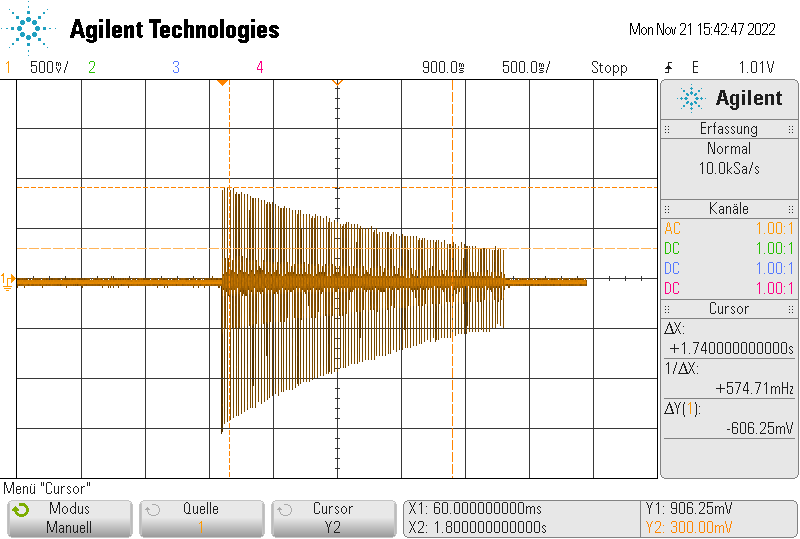
\includegraphics[width=0.6\textwidth]{python/data/scope_2.png}
  \caption{Das Signal das mit der Meiboom-Gill-Methode aufgenommen wurde.}
\label{img:Sig1}
\end{figure}


\noindent
Die ausgelesenen Spannungsamplituden sind in Tabelle \ref{tab:T2} dargestellt. 
Auf diesen Daten wird eine Funktion der Form
\begin{equation*}
  U\left(t\right) = U_0 \exp{\left(-\frac{t}{T_2}\right)} + U_2
\end{equation*}
gefittet. Dies ergibt die Parameter
\begin{align*}
  U_0 &= \SI{-0.887(023)}{\volt}\\
  T_2 &= \SI{1.976(097)}{\second}\\
  U_2 &= \SI{-0.064(026)}{\volt} \quad .
\end{align*}
Die Ausgleichsfunktion ist inklusive der ausgelesenen Maxima in Abbildung \ref{img:T2} grafisch dargestellt.


\begin{figure}[H]
  \centering
  \includegraphics[width=0.6\textwidth]{build/plots/T2.pdf}
  \caption{Die augelesenen Spannungsmaxima der $T2$-Messung gegen die halblogarithmischen Pulsabstände aufgetragen. 
  Zusätzlich ist noch der mit damit korrespondierende Fit aufgetragen.}
\label{img:T2}
\end{figure}


\subsection{Carr-Purcell-Methode}


\noindent
Eine alternative zur Meiboom-Gill-Methode ist die Carr-Purcell-Methode. Bei der der $\symup{\Delta} t_{90}$-Puls und der $\symup{\Delta} t_{180}$-Puls die gleiche Phase besitzen.
Eine Bestimmung der Relaxationszeit $T_2$ ist hieraus nicht möglich. Das gespeicherte Signal ist in Abbildung \ref{img:Sig2} zu finden.
\begin{figure}[H]
  \centering
  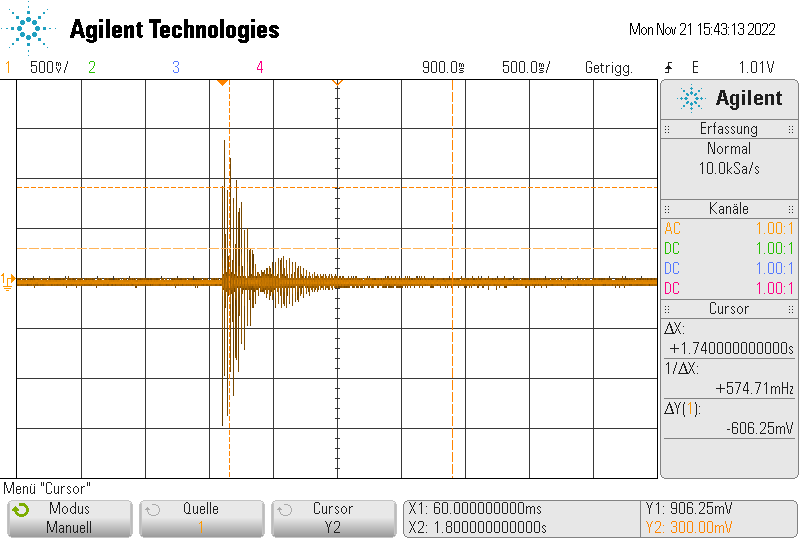
\includegraphics[width=0.6\textwidth]{python/data/scope_3.png}
  \caption{Das Signal das mit der Carr-Purcell-Methode aufgenommen wurde.}
\label{img:Sig2}
\end{figure}

\subsection{Bestimmung des Magnetfeldgradienten}


\noindent
Um die Stärke des Magnetfeldgradienten zu bestimmen wird das in Abbildung \ref{img:four1} dargestellte Echo fouriertransformiert. 
Das daraus erhaltene Frequenzspektrum ist in Abbildung \ref{img:four2} zu finden.
Dabei ist auch der Durchmesser des Probenröhrchens im Frequenzraum $d_\t{f}$ eingezeichnet.

\begin{figure}[H]
  \centering
  \includegraphics[width=0.6\textwidth]{build/plots/signal.pdf}
  \caption{Das Echo bei $\tau = \SI{5}{\milli\second}$, welches zur Bestimmung des Magnetfeldgradienten verwendet wird.}
\label{img:four1}
\end{figure}

\noindent
Für die Gradientenstärke ergibt sich damit
\begin{equation*}
  G = \frac{2\pi d_\text{f}}{\gamma d} = \SI{0.1203}{\tesla\per\metre} \quad.
\end{equation*}
Dabei ist  $d = \SI{4.2}{\milli\metre}$ \cite{V49} der Durchmesser des Probenröhrchens, $d_\text{f} \approx \SI{21467.6034}{\hertz}$ der Durchmesser im Frequenzraum und
$\gamma = \SI{2.67e8}{\per\second\tesla}$ \cite{gyro} das gyromagnetische Verhältnis für Protonen.

\begin{figure}[H]
  \centering
  \includegraphics[width=0.6\textwidth]{build/plots/echo_gradient.pdf}
  \caption{Das fouriertransformierten Echo inklusive der Breite des Halbkreises grafisch dargestellt. }
\label{img:four2}
\end{figure}


\subsection{Bestimmung der Diffusionskonstante}


\noindent Bevor über die Messwerte der Diffusionsmessung, welche in Tabelle \ref{tab:diff} aufgetragen sind, die Diffusionskonstante $D$ berechnet wird, 
wird quantitativ überprüft ob die Amplituden von $\tau^3$ abhängen.
Dafür wird, wie in Abbildung \ref{img:diff1} dargestellt,
\begin{equation*}
  \t{ln}(U(\tau)) - \frac{2\tau}{T_2}
\end{equation*}
gegen $\tau^3$ augetragen. Dabei wird ein linearer Abfall erwartet. Es ist zu erkennen, dass die Werte zwar einen linearen Verlauf besitzen, dieser aber einen Knick besitzt an dem sich die Steigung ändert.
Die Steigungen sind in vor und nach dem Knick allerdings annähernd linear.
\begin{table}[ht]
  \centering
  \small
  \caption{Die Messwerte der Spannungsamplituden $U$ und ihre korrespondierenden Pulsabstände $\tau$ für die Messung der Diffusionskonstante.}
  \label{tab:diff}
  \begin{tabular}{S [table-format=4.1] S [table-format=1.4] | S [table-format=4.1] S [table-format=1.4]}
   \toprule
   {$\tau \mathbin{\scalebox{1.5} / } \si{\milli\second}$} & {$\text{Spannungsamplitude} \mathbin{\scalebox{1.5} / } \si{\volt}$} &{$\tau \mathbin{\scalebox{1.5} / } \si{\milli\second}$} & {$\text{Spannungsamplitude} \mathbin{\scalebox{1.5} / } \si{\volt}$}\\
   \midrule 
  0.1 & 1.5   & 17   & 0.11  \\
  0.5 & 1.487 & 18   & 0.073 \\
  1   & 1.487 & 19   & 0.047 \\
  2.5 & 1.468 & 20   & 0.041 \\
  5   & 1.375 & 21   & 0.033 \\
  7.5 & 1.15  & 22   & 0.029 \\
 10   & 0.837 & 23   & 0.024 \\
 12.5 & 0.475 & 24   & 0.02  \\
 15   & 0.212 & 25   & 0.027 \\
 16   & 0.16   \\
 \bottomrule
  \end{tabular}
\end{table} 


\begin{figure}[H]
  \centering
  \includegraphics[width=0.6\textwidth]{build/plots/diff1.pdf}
  \caption{Die zur qualitativen Überprüfung der $\tau^3$-Konvergenz linear dargestellten Messdaten. }
\label{img:diff1}
\end{figure}


\noindent 
Nun wird auf die Spannungsamplituden eine Ausgleichsfunktion der Form 
\begin{equation*}
  U\left(\tau\right) = U_0 \exp{\left(-\frac{2\tau}{T_2}\right)} \exp{\left(-\frac{\tau^3}{T_D}\right)} + U_3
\end{equation*}
berechnet. Dabei ergeben sich
\begin{align*}
  U_0 &= \SI{1.4621(34)}{\volt}\\
  T_\t{D} &= \SI{1677.8387(141057)e3}{\milli\second^3}\\
  U_3 &= \SI{0.0260(23)}{\volt} \quad .
\end{align*}
Die Ausgleichsfunktion ist inklusive der Messwerte in Abbildung \ref{img:diff2} grafisch dargestellt.
Mit dem Fitparameter $T_\t{D}$ lässt sich die Diffusionskonstante $D$ zu 
\begin{equation*}
  D = \frac{3}{2\cdot T_\t{D} \gamma^2 G^2} = \SI{0.8665(73)e-9}{\metre^2\per\second}
\end{equation*}
berechnen. 


\begin{figure}[H]
  \centering
  \includegraphics[width=0.6\textwidth]{build/plots/diff2.pdf}
  \caption{Die Spannungsamplituden in Abhängigkeit von den korrespondierenden Pulsabständen inklusive der dazugehörigen Ausgleichsfunktion aufgetragen. }
\label{img:diff2}
\end{figure}



\subsection{Bestimmung des Molekülradius}


\noindent
Für die Bestimmung des Molekülradius $r$ wird die Stokes-Formel 
\begin{equation*}
  D = \frac{k_\text{B}T}{6\pi\eta r} \iff r = \frac{k_\text{B}T}{6 \pi\eta D}.
\end{equation*}
herangezogen. Dabei ist $\eta = \SI{1002}{\micro\pascal\second} $\cite{visko} die Viskosität von Wasser bei $T= \SI{20}{\degreeCelsius}$.
Für den Radius ergibt sich dabei 
\begin{equation*}
  r = \SI{1.755(15)e-11}{\metre} \quad .
\end{equation*}

\noindent
Zur Berechnung eines Vergleichwertes wird angenommen, dass die Moleküle in einer hexagonal dichtesten Kugelpackung angeordnet 
sind. Die Raumfüllung beträgt dort $\SI{74}{\percent}$. Mit einer Molekülmasse von $m = \frac{M_\text{mol}}{N_\text{A}} = \SI{2.99e-26}{\kilo\gram}$
und einer Dichte von $\rho=\SI{998}{\kilo\gram\per\metre^3}$\cite{visko} ergibt sich
\begin{equation*}
  r_\text{hcp} = \left(\frac{m\cdot 0.74}{\frac{4}{3}\pi\rho}\right)^{\frac{1}{3}} = \SI{1.74e-10}{\metre} \quad .
\end{equation*}
Dies bedeutet für das aus den Messungen eine relative Abweichung von $\increment r = \SI{89.92(8)}{\percent}$.

